\documentclass[presentation]{beamer}
\mode<presentation>{\usetheme{AMSBolognaFCrev}}

\usepackage[utf8]{inputenc}
\usepackage[T1]{fontenc}
\usepackage{booktabs}
\usepackage{array}
\usepackage{colortbl}
\usepackage{tabularx}
\usepackage{tikz}
\usepackage[ddmmyyyy]{datetime}
\usepackage[export]{adjustbox}
\usetikzlibrary{arrows.meta,positioning,shapes.geometric,fit,calc}

\renewcommand{\dateseparator}{/}
\newcommand{\sectiontitleframe}[1]{
\begin{frame}[plain,c]
\begin{center}
{\usebeamerfont{title}\usebeamercolor[fg]{title}#1}
\end{center}
\end{frame}
}

\tikzset{
    netbox/.style={draw, rounded corners, align=center, font=\scriptsize,
        minimum height=0.7cm, text width=2.0cm},
    netarrow/.style={-{Stealth[length=2mm]}, thick}
}

\title[Lesson 6]{Basic Networking and Firewalls}
\institute[Data Privacy and Security]{Healthcare Data Privacy and Security}
\author[\sspeaker{G. Pisano}]{\speaker{Giuseppe Pisano} \\\href{mailto:g.pisano@unibo.it}{g.pisano@unibo.it}}
\date[August, 2026]{August, 2026}
%
\titlegraphic{
\begin{center}
    
\includegraphics[width=0.35\textwidth, valign=c]{logos/intestazione.png}
    
\includegraphics[width=0.16\textwidth, valign=c]{logos/unibo_logo_2.png}
    
\includegraphics[width=0.11\textwidth, valign=c]{logos/makeni_logo_2.png}
    
\includegraphics[width=0.20\textwidth, valign=c]{logos/cuamm_logo_png.png}
\end{center}
\centering
\tiny{S.K.I.L.L.E.D --- AID013244/04/2\\Strategic Knowledge and Inclusive Lifelong Learning in the health sector for youth Employability and Development}
}

\newcommand{\scenario}{St. Isidore Hospital}
\newcommand{\takeawaysframe}[2]{
\begin{frame}[c]{Recap: \insertsection}
\begin{block}{Takeaways}
#1
\end{block}
\begin{exampleblock}{In \scenario}
#2
\end{exampleblock}
\end{frame}
}

\begin{document}

\setbeamertemplate{frametitle}
{
    \nointerlineskip
    \begin{beamercolorbox}[sep=0.3cm,ht=2.2em,wd=\paperwidth]{frametitle}
        \vbox{}\vskip-2ex%
        \strut\insertframetitle\hfill\raisebox{-0.2\height}{
\includegraphics[width=2cm]{logos/cuamm_logo_png.png}}\strut
        \vskip-0.8ex%
    \end{beamercolorbox}
}

\begin{frame}[allowframebreaks]
\titlepage
\end{frame}

\begin{frame}[c,allowframebreaks]{Roadmap}
\tableofcontents[hideallsubsections]
\end{frame}

\begin{frame}[c]{How This Lesson Progresses}
\begin{block}{Learning path}
We start from the language of networks: \textbf{hosts}, \textbf{addresses}, \textbf{packets},
\textbf{ports}, and \textbf{protocols}. Then we move to \textbf{hospital network zones},
\textbf{firewalls}, \textbf{DMZs}, \textbf{VPNs}, a \textbf{hands-on firewall lab}, and finally an optional view of
\textbf{cloud computing}.
\end{block}

\begin{exampleblock}{Hospital storyline}
\scenario{} operates an EHR, laboratory system, pharmacy system, imaging archive, patient portal,
guest Wi-Fi, medical devices, remote access for clinicians, and some cloud services. Networking
decides which systems can reach each other; firewalls enforce that decision.
\end{exampleblock}
\end{frame}

\begin{frame}[c]{Connection with Other Lessons}
\begin{block}{Where this fits}
Networking is the map on which many security controls operate. Firewalls control traffic paths,
authentication protects remote entry points, encryption protects communication, and access control
limits what authenticated users can do after they reach an application.
\end{block}

\begin{itemize}
    \item \textbf{Encryption}: TLS, VPNs, and IPsec protect traffic across untrusted networks.
    \item \textbf{Access control}: network segmentation reduces which systems can even be contacted.
    \item \textbf{Authentication}: VPNs, proxies, cloud consoles, and administrative interfaces need strong identity checks.
    \item \textbf{Privacy and compliance}: network security supports confidentiality, integrity, availability, and incident containment.
\end{itemize}
\end{frame}

\section{Networking Foundations}
\sectiontitleframe{Networking Foundations}

\begin{frame}[c]{Section Context: Networking Foundations}
\begin{block}{What we are talking about}
A network lets systems exchange data. Security begins by understanding what communicates, through
which path, using which protocol, and for what operational purpose.
\end{block}

\begin{exampleblock}{Hospital lens}
When a ward workstation opens an EHR page, it may use DNS, IP routing, TCP, TLS, HTTP, database
connections, authentication services, and logging systems. A firewall rule sees only part of that
story unless the architecture is documented.
\end{exampleblock}
\end{frame}

\begin{frame}[c]{Hosts, Clients, and Servers}
\begin{block}{Host}
A host is any device with a network identity: workstation, server, printer, phone, medical device,
container, virtual machine, or firewall interface.
\end{block}

\begin{block}{Client and server}
A client initiates a request. A server waits for requests on a network address and port. The same
machine can be a client in one flow and a server in another.
\end{block}

\begin{exampleblock}{Hospital example}
A lab analyzer is a client when it sends results to the laboratory system. The laboratory system is
a server for the analyzer, but a client when it forwards verified results to the EHR.
\end{exampleblock}
\end{frame}

\begin{frame}[c]{IP Addresses}
\begin{block}{Addressing}
IP gives hosts logical addresses so packets can be routed across interconnected networks
\cite{rfc791}. IPv4 addresses look like \texttt{192.168.10.42}; IPv6 addresses are longer and written
in hexadecimal groups.
\end{block}

\begin{exampleblock}{Hospital example}
The EHR application server may live at \texttt{10.20.5.15}. A ward workstation at
\texttt{10.30.2.44} can reach it only if routing and firewall policy allow the path.
\end{exampleblock}
\end{frame}

\begin{frame}[c]{Private and Public Addresses}
\begin{block}{Private addresses}
Hospitals usually use private address ranges internally, such as \texttt{10.0.0.0/8},
\texttt{172.16.0.0/12}, or \texttt{192.168.0.0/16}. These are not directly routed on the public
Internet.
\end{block}

\begin{block}{Public addresses}
Internet-facing services need public reachability, often through a firewall, load balancer, reverse
proxy, or cloud edge service.
\end{block}
\end{frame}

\begin{frame}[c]{Subnets}
\begin{block}{Core idea}
A subnet groups addresses that belong to the same local network segment. CIDR notation describes
the network size: \texttt{10.30.2.0/24} means addresses from \texttt{10.30.2.0} to
\texttt{10.30.2.255}.
\end{block}

\begin{exampleblock}{Hospital example}
St. Isidore may assign \texttt{10.10.0.0/24} to servers, \texttt{10.20.0.0/24} to clinical
workstations, \texttt{10.30.0.0/24} to medical devices, and \texttt{10.90.0.0/24} to guest Wi-Fi.
\end{exampleblock}
\end{frame}

\begin{frame}[c]{Ports and Services}
\begin{block}{Port}
A port identifies a service endpoint on a host. The address tells us which host; the port tells us
which application or service on that host.
\end{block}

\begin{exampleblock}{Hospital example}
The same server might expose HTTPS on port \texttt{443}, SSH administration on port \texttt{22},
and a database listener on port \texttt{5432}. A good firewall policy does not treat these as the
same risk.
\end{exampleblock}
\end{frame}

\begin{frame}[c]{Common Ports}
\small
\begin{tabularx}{\textwidth}{@{}p{0.18\textwidth}p{0.22\textwidth}X@{}}
\toprule
\textbf{Port} & \textbf{Protocol} & \textbf{Typical use} \\
\midrule
53 & DNS & Name resolution \\
80 / 443 & HTTP / HTTPS & Web applications and APIs \\
25 / 587 & SMTP & Email relay and submission \\
22 & SSH & Remote administration \\
3389 & RDP & Windows remote desktop \\
5432 / 3306 & PostgreSQL / MySQL & Database access \\
\bottomrule
\end{tabularx}

\begin{block}{Security point}
Opening a port means exposing a service. The risk depends on the service, who can reach it, and how
it is authenticated, patched, and monitored.
\end{block}
\end{frame}

\begin{frame}[c]{Packets and Flows}
\begin{block}{Packet}
A packet carries headers and payload. Headers contain delivery information such as source,
destination, protocol, and ports. Payload contains the data being carried.
\end{block}

\begin{block}{Flow}
A flow is the conversation formed by related packets, such as a workstation connecting to the EHR
over HTTPS.
\end{block}

\begin{exampleblock}{Hospital example}
A firewall may log a flow as: source \texttt{10.20.0.45}, destination \texttt{10.10.0.12}, protocol
TCP, port \texttt{443}, action allowed.
\end{exampleblock}
\end{frame}

\begin{frame}[c]{Scheme: From User Action to Network Flow}
\begin{center}
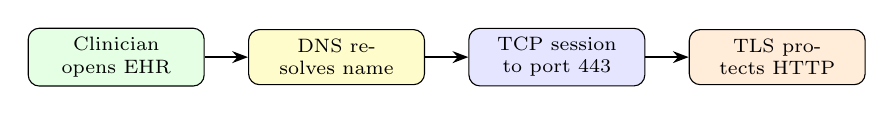
\begin{tikzpicture}[node distance=0.55cm]
\node[netbox, fill=green!10] (user) {Clinician opens EHR};
\node[netbox, right=of user, fill=yellow!20] (dns) {DNS resolves name};
\node[netbox, right=of dns, fill=blue!10] (tcp) {TCP session to port 443};
\node[netbox, right=of tcp, fill=orange!15] (tls) {TLS protects HTTP};
\draw[netarrow] (user) -- (dns);
\draw[netarrow] (dns) -- (tcp);
\draw[netarrow] (tcp) -- (tls);
\end{tikzpicture}
\end{center}

\begin{block}{Reading the scheme}
A simple click in the browser becomes multiple network events. Security controls may operate at
different points in that path.
\end{block}
\end{frame}

\begin{frame}[c]{TCP and UDP}
\begin{block}{TCP}
TCP is connection-oriented. It establishes a session, tracks sequence numbers, retransmits lost data,
and is common for web, email, remote administration, and many databases \cite{rfc9293}.
\end{block}

\begin{block}{UDP}
UDP is connectionless. It has less overhead and is common for DNS, some real-time traffic, and
protocols where the application handles reliability \cite{rfc768}.
\end{block}
\end{frame}

\begin{frame}[c]{DNS, DHCP, NAT}
\begin{block}{DNS}
DNS translates names into addresses. If DNS fails or is poisoned, users may not reach the correct
service.
\end{block}

\begin{block}{DHCP}
DHCP assigns network configuration automatically, such as IP address, gateway, and DNS server.
\end{block}

\begin{block}{NAT}
Network Address Translation maps internal addresses to other addresses, often allowing many private
hosts to share public Internet connectivity.
\end{block}
\end{frame}

\takeawaysframe{
\begin{itemize}
    \item Networks are built from hosts, addresses, ports, protocols, packets, and flows.
    \item Security decisions should be based on documented communication needs.
    \item A network path is not automatically safe just because the application login works.
\end{itemize}
}{
The hospital must know which systems talk to which services before it can write meaningful firewall
rules or detect suspicious traffic.
}

\section{Hospital Network Architecture}
\sectiontitleframe{Hospital Network Architecture}

\begin{frame}[c]{Section Context: Hospital Network Architecture}
\begin{block}{What we are talking about}
Enterprise networks evolved from centralized systems to LANs, interconnected internal networks, WANs,
Internet connectivity, remote access, and cloud services. Each step increases reachability and the
need for controlled boundaries.
\end{block}

\begin{exampleblock}{Hospital lens}
St. Isidore no longer has one mainframe and terminals. It has clinical workstations, servers,
medical devices, mobile devices, partner connections, public services, and cloud platforms.
\end{exampleblock}
\end{frame}

\begin{frame}[c]{LAN, WAN, and Internet}
\begin{block}{LAN}
A Local Area Network connects systems in a limited area, such as a hospital building, ward, or data
center.
\end{block}

\begin{block}{WAN}
A Wide Area Network connects sites across larger distances, such as a main hospital, rural clinic,
and administrative office.
\end{block}

\begin{block}{Internet}
Internet connectivity is operationally essential but exposes internal resources to external threats
unless carefully mediated.
\end{block}
\end{frame}

\begin{frame}[c]{Network Zones}
\begin{block}{Zone}
A zone is a group of systems with similar trust level, exposure, and security requirements.
\end{block}

\begin{exampleblock}{Hospital example}
Useful zones include public services, DMZ, clinical workstations, servers, medical devices, guest
Wi-Fi, administration, backup, and security monitoring.
\end{exampleblock}
\end{frame}

\begin{frame}[c]{Scheme: Hospital Zones}
\begin{center}
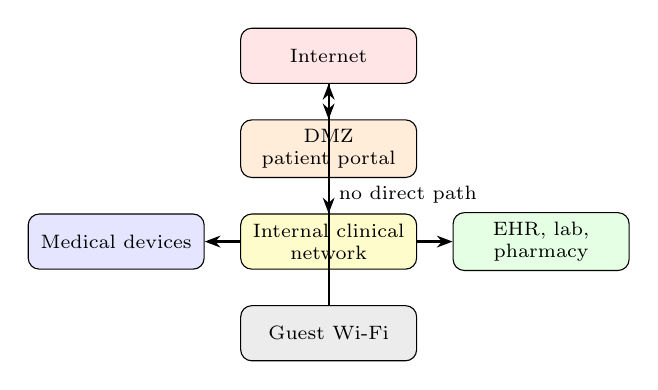
\begin{tikzpicture}[node distance=0.45cm]
\node[netbox, fill=red!10] (internet) {Internet};
\node[netbox, below=of internet, fill=orange!15] (dmz) {DMZ\\patient portal};
\node[netbox, below=of dmz, fill=yellow!20] (core) {Internal clinical network};
\node[netbox, left=of core, fill=blue!10] (devices) {Medical devices};
\node[netbox, right=of core, fill=green!10] (servers) {EHR, lab, pharmacy};
\node[netbox, below=of core, fill=gray!15] (guest) {Guest Wi-Fi};
\draw[netarrow] (internet) -- (dmz);
\draw[netarrow] (dmz) -- (core);
\draw[netarrow] (core) -- (devices);
\draw[netarrow] (core) -- (servers);
\draw[netarrow] (guest) -- node[right,font=\scriptsize]{no direct path} (internet);
\end{tikzpicture}
\end{center}

\begin{block}{Design point}
Zones reduce blast radius. A compromised guest phone should not be able to scan medication cabinets
or database servers.
\end{block}
\end{frame}

\begin{frame}[c]{Segmentation}
\begin{block}{Core idea}
Segmentation separates systems so that compromise in one area does not automatically imply access to
all other areas.
\end{block}

\begin{exampleblock}{Hospital example}
Imaging devices may need to send studies to PACS, but they should not browse the payroll database,
reach backup servers, or initiate arbitrary outbound Internet connections.
\end{exampleblock}
\end{frame}

\begin{frame}[c]{Choke Points}
\begin{block}{Firewall placement}
A firewall should create a controlled point where traffic can be allowed, denied, logged, and
investigated. The traditional goal is that all traffic between zones passes through the firewall.
\end{block}

\begin{exampleblock}{Hospital example}
If the patient portal can talk directly to the EHR database without crossing a monitored control
point, the hospital loses visibility and containment.
\end{exampleblock}
\end{frame}

\takeawaysframe{
\begin{itemize}
    \item Hospital networks should be described as zones and flows, not only as devices.
    \item Segmentation supports safety, privacy, resilience, and incident containment.
    \item Choke points matter because controls and logs need a place to operate.
\end{itemize}
}{
St. Isidore should separate public services, clinical systems, devices, guest access, and
administration before deciding detailed firewall rules.
}

\section{Firewall Fundamentals}
\sectiontitleframe{Firewall Fundamentals}

\begin{frame}[c]{Section Context: Firewall Fundamentals}
\begin{block}{What we are talking about}
A firewall protects a host or network by controlling network traffic according to security policy. It
is not a complete security system, but it is a central enforcement and monitoring point.
\end{block}

\begin{exampleblock}{Hospital lens}
The hospital firewall does not know whether a diagnosis is correct, but it can prevent the guest
Wi-Fi network from reaching the EHR database port.
\end{exampleblock}
\end{frame}

\begin{frame}[c]{Firewall Goals}
\begin{block}{Classic design goals}
\begin{itemize}
    \item All relevant traffic should pass through the firewall.
    \item Only traffic authorized by policy should pass.
    \item The firewall itself should be hardened and resistant to compromise.
\end{itemize}
\end{block}

\begin{exampleblock}{Hospital example}
Internet users may reach the public patient portal, but not internal laboratory analyzers or the
database backend.
\end{exampleblock}
\end{frame}

\begin{frame}[c]{Firewall Policy}
\begin{block}{Policy question}
Which traffic should be allowed, between which sources and destinations, using which protocols,
ports, users, applications, time windows, and logging requirements?
\end{block}

\begin{exampleblock}{Hospital example}
Allow clinical workstations to reach the EHR on HTTPS. Allow the EHR application server to reach
the database. Deny direct workstation-to-database access.
\end{exampleblock}
\end{frame}

\begin{frame}[c]{Positive and Negative Filtering}
\begin{block}{Positive filtering}
Allow only traffic that matches approved criteria. This is conservative: default deny, then add what
the hospital needs.
\end{block}

\begin{block}{Negative filtering}
Block traffic that matches forbidden criteria. This is easier at first, but it assumes administrators
know every dangerous pattern in advance.
\end{block}
\end{frame}

\begin{frame}[c]{Default Action}
\begin{block}{Default deny}
Everything not explicitly allowed is blocked. This is usually preferred for sensitive healthcare
networks.
\end{block}

\begin{block}{Default allow}
Everything not explicitly blocked is allowed. This may reduce support tickets, but it often leaves
unexpected paths open.
\end{block}
\end{frame}

\begin{frame}[c]{Firewall Limitations}
\begin{block}{A firewall cannot}
\begin{itemize}
    \item protect against traffic that bypasses it;
    \item stop every insider threat;
    \item inspect traffic it cannot see or decrypt;
    \item compensate for unpatched exposed services;
    \item protect a laptop infected outside the hospital before it reconnects internally.
\end{itemize}
\end{block}
\end{frame}

\takeawaysframe{
\begin{itemize}
    \item Firewalls enforce network policy at controlled points.
    \item Default deny is safer for clinical and administrative systems.
    \item Firewalls reduce risk, but do not replace patching, authentication, endpoint security, and monitoring.
\end{itemize}
}{
The hospital should use firewalls to make expected traffic explicit and unexpected traffic visible.
}

\section{Packet Filtering}
\sectiontitleframe{Packet Filtering}

\begin{frame}[c]{Section Context: Packet Filtering}
\begin{block}{What we are talking about}
Packet filtering firewalls decide whether to forward or discard packets based on information in
network and transport headers.
\end{block}

\begin{exampleblock}{Hospital lens}
A packet filter can allow \texttt{10.20.0.0/24} to reach the EHR web server on TCP port
\texttt{443}, while denying guest Wi-Fi access to the same destination.
\end{exampleblock}
\end{frame}

\begin{frame}[c]{What Packet Filters Inspect}
\begin{block}{Typical fields}
\begin{itemize}
    \item source and destination IP address;
    \item protocol, such as TCP, UDP, or ICMP;
    \item source and destination port;
    \item input or output interface;
    \item selected TCP flags, such as ACK.
\end{itemize}
\end{block}
\end{frame}

\begin{frame}[c]{Rule Order Matters}
\begin{block}{Top-down evaluation}
Firewall rules are usually evaluated from top to bottom. The first matching rule decides the action.
The final rule should make the default action explicit.
\end{block}

\begin{exampleblock}{Hospital example}
If a broad ``allow clinical network to any database port'' rule appears before a narrow deny rule,
the narrow deny rule may never be reached.
\end{exampleblock}
\end{frame}

\begin{frame}[c]{Example Rule Set}
\small
\begin{tabularx}{\textwidth}{@{}p{0.09\textwidth}p{0.23\textwidth}p{0.23\textwidth}p{0.18\textwidth}X@{}}
\toprule
\textbf{\#} & \textbf{Source} & \textbf{Destination} & \textbf{Service} & \textbf{Action} \\
\midrule
1 & Clinical LAN & EHR web & TCP 443 & Allow \\
2 & EHR web & EHR DB & TCP 5432 & Allow \\
3 & Clinical LAN & EHR DB & TCP 5432 & Deny \\
4 & Guest Wi-Fi & Internal nets & Any & Deny \\
5 & Any & Any & Any & Deny \\
\bottomrule
\end{tabularx}

\begin{block}{Reading the table}
Users reach the application, not the database. The application reaches the database. Guest Wi-Fi is
kept out of internal networks.
\end{block}
\end{frame}

\begin{frame}[c]{SMTP Example: Why Details Matter}
\begin{block}{Problem}
Simple SMTP rules may allow inbound traffic to high-numbered client ports or allow any internal host
to send mail directly to the Internet.
\end{block}

\begin{exampleblock}{Hospital example}
If every workstation can send SMTP to the Internet, malware on one workstation can send spam or
exfiltrate data. A safer policy forces outbound mail through the hospital mail gateway.
\end{exampleblock}
\end{frame}

\begin{frame}[c]{Packet Filtering Strengths}
\begin{block}{Advantages}
\begin{itemize}
    \item simple and fast;
    \item transparent to users;
    \item suitable for hardware implementation;
    \item useful for broad segmentation and baseline policy.
\end{itemize}
\end{block}
\end{frame}

\begin{frame}[c]{Packet Filtering Weaknesses}
\begin{block}{Limitations}
\begin{itemize}
    \item it does not understand application functions;
    \item logging is limited to inspected fields unless configured carefully;
    \item advanced user authentication is difficult at packet level;
    \item TCP/IP quirks and fragmentation can create bypass risks;
    \item misconfiguration is a major security flaw.
\end{itemize}
\end{block}
\end{frame}

\begin{frame}[c]{Attacks on Packet Filters}
\begin{block}{IP spoofing}
An attacker sends packets with a forged internal source address. Countermeasure: drop packets with
internal source addresses arriving from external interfaces.
\end{block}

\begin{block}{Source routing}
An attacker tries to specify the packet route to bypass policy. Countermeasure: block source-routing
options.
\end{block}

\begin{block}{Tiny fragments}
An attacker fragments packets so the first fragment hides important TCP header fields. Countermeasure:
require enough header information before accepting fragments.
\end{block}
\end{frame}

\takeawaysframe{
\begin{itemize}
    \item Packet filters are fast and useful, but they see limited context.
    \item Rule order and default action are security-critical.
    \item Header tricks, broad rules, and weak logging can undermine the design.
\end{itemize}
}{
St. Isidore should use packet filtering for clear zone boundaries, but not rely on it to understand
clinical application behavior.
}

\section{Stateful and Proxy Firewalls}
\sectiontitleframe{Stateful and Proxy Firewalls}

\begin{frame}[c]{Section Context: Stateful and Proxy Firewalls}
\begin{block}{What we are talking about}
Traditional packet filters inspect each packet in isolation. Stateful and proxy firewalls add more
context: connection state, transport sessions, application behavior, or user identity.
\end{block}

\begin{exampleblock}{Hospital lens}
The firewall should know whether an inbound packet is part of a legitimate existing connection from
the EHR server, or an unsolicited attempt from the Internet.
\end{exampleblock}
\end{frame}

\begin{frame}[c]{Stateful Packet Inspection}
\begin{block}{Core idea}
A stateful firewall records active connections. It allows return traffic only when it matches a
known established flow.
\end{block}

\begin{exampleblock}{Hospital example}
If a pharmacy workstation opens an HTTPS session to an update service, return packets for that
session are allowed. Unsolicited inbound packets to random high ports are denied.
\end{exampleblock}
\end{frame}

\begin{frame}[c]{Scheme: Stateful Firewall}
\begin{center}
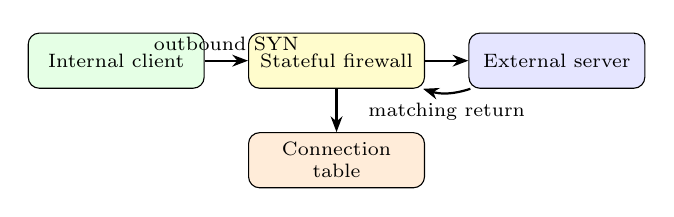
\begin{tikzpicture}[node distance=0.55cm]
\node[netbox, fill=green!10] (client) {Internal client};
\node[netbox, right=of client, fill=yellow!20] (fw) {Stateful firewall};
\node[netbox, right=of fw, fill=blue!10] (server) {External server};
\node[netbox, below=of fw, fill=orange!15] (table) {Connection table};
\draw[netarrow] (client) -- node[above,font=\scriptsize]{outbound SYN} (fw);
\draw[netarrow] (fw) -- (server);
\draw[netarrow] (fw) -- (table);
\draw[netarrow] (server) to[bend left=18] node[below,font=\scriptsize]{matching return} (fw);
\end{tikzpicture}
\end{center}
\end{frame}

\begin{frame}[c]{Application-Level Gateway}
\begin{block}{Application proxy}
An application-level gateway understands a specific application protocol. It can authenticate users,
inspect application commands, enforce protocol-specific policy, and produce richer logs.
\end{block}

\begin{exampleblock}{Hospital example}
A web proxy can allow staff to browse approved medical resources while blocking known malicious
sites, suspicious downloads, or unauthorized upload destinations.
\end{exampleblock}
\end{frame}

\begin{frame}[c]{Application Proxy Trade-Off}
\begin{block}{Benefit}
The proxy can make more meaningful decisions than a packet filter because it sees application-level
semantics.
\end{block}

\begin{block}{Cost}
The proxy adds overhead and complexity. It splits communication into two connections: client to
proxy, and proxy to remote service.
\end{block}
\end{frame}

\begin{frame}[c]{Circuit-Level Gateway}
\begin{block}{Core idea}
A circuit-level gateway also creates two TCP connections, but it focuses on transport-level session
control rather than inspecting application content.
\end{block}

\begin{exampleblock}{Hospital example}
A SOCKS gateway can decide whether a workstation may establish an outbound connection, without
understanding the full application protocol running through that connection.
\end{exampleblock}
\end{frame}

\begin{frame}[c]{Comparing Firewall Types}
\small
\begin{tabularx}{\textwidth}{@{}p{0.25\textwidth}p{0.28\textwidth}X@{}}
\toprule
\textbf{Type} & \textbf{Sees} & \textbf{Good for} \\
\midrule
Packet filter & IPs, ports, protocol, interface & Fast baseline filtering \\
Stateful firewall & Packet fields plus connection state & Safer return traffic handling \\
Circuit gateway & Transport-level sessions & Controlled outbound connectivity \\
Application proxy & Application protocol and sometimes user identity & Deep policy and better logs \\
\bottomrule
\end{tabularx}
\end{frame}

\takeawaysframe{
\begin{itemize}
    \item Stateful firewalls reduce risks created by dynamic client ports.
    \item Application proxies can enforce richer policy, but add overhead.
    \item Firewall type should match the policy question being asked.
\end{itemize}
}{
St. Isidore may use stateful firewalls between zones and application proxies for Internet browsing,
mail, or exposed web services.
}

\section{Deployment Patterns}
\sectiontitleframe{Deployment Patterns}

\begin{frame}[c]{Section Context: Deployment Patterns}
\begin{block}{What we are talking about}
Firewall value depends on placement. The same rule behaves differently at the Internet edge, between
internal zones, on a server host, or inside a cloud security group.
\end{block}

\begin{exampleblock}{Hospital lens}
An edge firewall protects from the Internet, but it may not stop a compromised ward workstation from
reaching a database unless internal segmentation also exists.
\end{exampleblock}
\end{frame}

\begin{frame}[c]{Bastion Host}
\begin{block}{Definition}
A bastion host is a hardened system identified as a critical security point. It often hosts an
application proxy, circuit gateway, jump service, or administrative entry point.
\end{block}

\begin{block}{Hardening}
Install only essential services, restrict privileges, protect configuration, keep executable code
read-only where possible, log access carefully, and monitor changes.
\end{block}
\end{frame}

\begin{frame}[c]{Host-Based and Personal Firewalls}
\begin{block}{Host-based firewall}
A software firewall protects one server or workstation. It can apply rules tailored to that host's
role, independent of network topology.
\end{block}

\begin{block}{Personal firewall}
A lighter endpoint firewall blocks unexpected inbound access and may monitor outbound application
activity to detect malware or unsafe software.
\end{block}
\end{frame}

\begin{frame}[c]{DMZ}
\begin{block}{Definition}
A demilitarized zone is a network segment for systems that must be reachable from outside but should
not sit directly inside the trusted internal network.
\end{block}

\begin{exampleblock}{Hospital example}
The patient portal reverse proxy belongs in the DMZ. The EHR database does not.
\end{exampleblock}
\end{frame}

\begin{frame}[c]{Scheme: DMZ with Internal Firewall}
\begin{center}
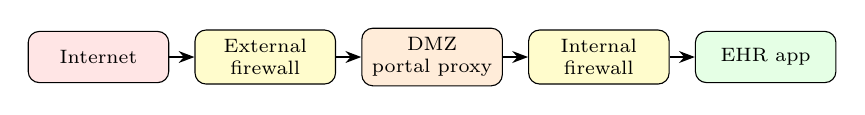
\begin{tikzpicture}[
    node distance=0.32cm,
    smallbox/.style={draw, rounded corners, align=center, font=\scriptsize,
        minimum height=0.65cm, text width=1.55cm}
]
\node[smallbox, fill=red!10] (internet) {Internet};
\node[smallbox, right=of internet, fill=yellow!20] (fw1) {External firewall};
\node[smallbox, right=of fw1, fill=orange!15] (dmz) {DMZ\\portal proxy};
\node[smallbox, right=of dmz, fill=yellow!20] (fw2) {Internal firewall};
\node[smallbox, right=of fw2, fill=green!10] (internal) {EHR app};
\draw[netarrow] (internet) -- (fw1);
\draw[netarrow] (fw1) -- (dmz);
\draw[netarrow] (dmz) -- (fw2);
\draw[netarrow] (fw2) -- (internal);
\end{tikzpicture}
\end{center}

\begin{block}{Reading the scheme}
The DMZ is not trusted like the internal network. If a DMZ host is compromised, the internal firewall
still limits what the attacker can reach next.
\end{block}
\end{frame}

\begin{frame}[c]{Distributed Firewalling}
\begin{block}{Core idea}
Modern networks combine edge firewalls, internal firewalls, host-based rules, cloud security groups,
and endpoint controls under one administrative policy.
\end{block}

\begin{exampleblock}{Hospital example}
Even if a workstation is inside the hospital building, its local firewall can still block unexpected
incoming connections from another compromised workstation.
\end{exampleblock}
\end{frame}

\begin{frame}[c]{Monitoring and Logs}
\begin{block}{Why logs matter}
Firewall logs help reconstruct attempted connections, denied traffic, unusual flows, scans, policy
violations, and possible compromise.
\end{block}

\begin{block}{Operational need}
Logs should be aggregated with alerts and other telemetry. Isolated firewall logs are useful; linked
firewall, identity, endpoint, and application logs are much more useful.
\end{block}
\end{frame}

\takeawaysframe{
\begin{itemize}
    \item Placement determines what a firewall can see and enforce.
    \item DMZs protect public-facing services without placing them fully inside the trusted network.
    \item Distributed firewalling and log aggregation are necessary in modern environments.
\end{itemize}
}{
The hospital should not rely only on one Internet-edge firewall. Internal segmentation and host-based
controls reduce lateral movement.
}

\section{VPNs and Secure Remote Access}
\sectiontitleframe{VPNs and Secure Remote Access}

\begin{frame}[c]{Section Context: VPNs and Secure Remote Access}
\begin{block}{What we are talking about}
A VPN uses cryptography and authentication to create a protected connection across an untrusted
network. It is useful for remote sites and remote users, but it also creates an entry point into the
organization.
\end{block}

\begin{exampleblock}{Hospital lens}
Doctors on call, external specialists, remote clinics, and administrators may need access from
outside the hospital. The VPN must protect traffic and control who enters.
\end{exampleblock}
\end{frame}

\begin{frame}[c]{What a VPN Provides}
\begin{block}{Confidentiality}
Traffic is encrypted so outsiders cannot easily read it.
\end{block}

\begin{block}{Authentication}
The VPN endpoint authenticates users, devices, sites, or gateways before allowing traffic.
\end{block}

\begin{block}{Integrity}
Cryptographic checks help detect modification of protected traffic.
\end{block}
\end{frame}

\begin{frame}[c]{IPsec Scenario}
\begin{block}{Site-to-site VPN}
Two hospital sites can use IPsec gateways to protect traffic across a public WAN. Internal traffic
may be ordinary IP inside each LAN, while traffic crossing the public network is encrypted.
\end{block}

\begin{exampleblock}{Hospital example}
The rural clinic sends laboratory orders to the main hospital. IPsec protects the inter-site path,
but internal firewalls still decide which applications the clinic can reach.
\end{exampleblock}
\end{frame}

\begin{frame}[c]{Scheme: Site-to-Site VPN}
\begin{center}
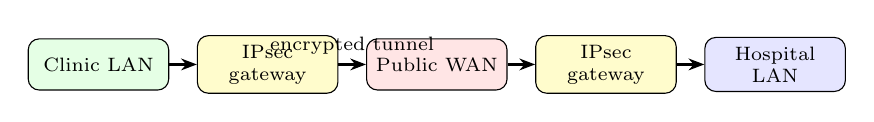
\begin{tikzpicture}[
    node distance=0.35cm,
    smallbox/.style={draw, rounded corners, align=center, font=\scriptsize,
        minimum height=0.65cm, text width=1.55cm}
]
\node[smallbox, fill=green!10] (clinic) {Clinic LAN};
\node[smallbox, right=of clinic, fill=yellow!20] (gw1) {IPsec gateway};
\node[smallbox, right=of gw1, fill=red!10] (wan) {Public WAN};
\node[smallbox, right=of wan, fill=yellow!20] (gw2) {IPsec gateway};
\node[smallbox, right=of gw2, fill=blue!10] (hospital) {Hospital LAN};
\draw[netarrow] (clinic) -- (gw1);
\draw[netarrow] (gw1) -- node[above,font=\scriptsize]{encrypted tunnel} (wan);
\draw[netarrow] (wan) -- (gw2);
\draw[netarrow] (gw2) -- (hospital);
\end{tikzpicture}
\end{center}
\end{frame}

\begin{frame}[c]{VPN Placement}
\begin{block}{Inspection problem}
If traffic is encrypted before it reaches an internal firewall, the firewall may not be able to
inspect application details. VPN placement affects visibility and control.
\end{block}

\begin{exampleblock}{Hospital example}
If a remote user's VPN tunnel drops them directly into the clinical network, the hospital may have
less segmentation than expected. A better design terminates VPN access in a controlled zone.
\end{exampleblock}
\end{frame}

\begin{frame}[c]{VPN Is Not Full Trust}
\begin{block}{Common mistake}
Authenticating to the VPN should not mean unrestricted internal access.
\end{block}

\begin{exampleblock}{Hospital example}
An external radiologist may need PACS and imaging reports, not payroll, pharmacy stock systems, or
domain controller administration.
\end{exampleblock}
\end{frame}

\takeawaysframe{
\begin{itemize}
    \item VPNs protect traffic over untrusted networks using cryptography and authentication.
    \item VPN placement affects firewall visibility.
    \item Remote access should still be segmented and least-privilege.
\end{itemize}
}{
St. Isidore should treat VPN as a secure path to controlled services, not as a magic door into the
whole hospital network.
}

\section{Hands-On Lab: Firewall Simulation}
\sectiontitleframe{Hands-On Lab}

\begin{frame}[c]{Section Context: Firewall Simulation Lab}
\begin{block}{What we are talking about}
Before using a real firewall, it helps to practice with a controlled model. The lab uses Python to
simulate packets, zones, firewall rules, stateful replies, default-deny behavior, and firewall logs.
\end{block}

\begin{exampleblock}{Hospital lens}
St. Isidore wants to check whether doctors can reach the EHR, whether guest Wi-Fi is isolated,
whether the EHR application can reach its database, and whether the database blocks direct access
from workstations.
\end{exampleblock}
\end{frame}

\begin{frame}[c]{Lab Tool Choice}
\begin{block}{Notebook simulator}
The notebook in \texttt{lesson-06/examples} is a \textbf{teaching firewall}. It does not protect the
computer running it. It makes the decision process visible: each packet is matched against ordered
rules, and every decision is logged.
\end{block}

\begin{block}{Realistic next steps}
\textbf{Mininet} can emulate hosts, switches, links, and Linux network stacks on one machine, while
\textbf{Scapy} can craft and inspect packets. They are powerful, but they usually require root or a
Linux VM, so they fit better after the concepts are clear.
\end{block}
\end{frame}

\begin{frame}[c]{Lab 1: Packet Filtering}
\begin{block}{Goal}
Model the hospital network as zones and write rules that describe expected traffic.
\end{block}

\begin{itemize}
    \item allow clinical workstations to reach the EHR web service on TCP 443;
    \item allow only the EHR application server to reach the EHR database on TCP 5432;
    \item block guest Wi-Fi from internal services;
    \item log the first rule that matched each packet.
\end{itemize}
\end{frame}

\begin{frame}[c]{Lab 2: Rule Order and Default Deny}
\begin{block}{Goal}
See why firewall policy is not just a list of wishes. It is an ordered decision procedure.
\end{block}

\begin{exampleblock}{Hospital example}
If a broad allow rule is placed before a deny rule, the deny rule may never run. The lab changes the
order and shows how the same packet receives a different decision.
\end{exampleblock}
\end{frame}

\begin{frame}[c]{Lab 3: Stateful Replies}
\begin{block}{Goal}
Compare a stateless filter with a stateful firewall.
\end{block}

\begin{exampleblock}{Hospital example}
A doctor opens an HTTPS connection to the EHR. The request goes from the clinical LAN to the EHR
server, but the response comes back in the opposite direction. A stateful firewall can allow the
reply because it belongs to an established flow.
\end{exampleblock}
\end{frame}

\begin{frame}[c]{Lab 4: Reading Firewall Logs}
\begin{block}{Goal}
Use logs to explain policy behavior instead of guessing.
\end{block}

\begin{itemize}
    \item identify which rule allowed or denied each connection;
    \item count denied attempts by source zone;
    \item find policy mistakes, such as direct database access from workstations;
    \item connect log evidence to segmentation decisions.
\end{itemize}
\end{frame}

\takeawaysframe{
\begin{itemize}
    \item A firewall policy is an executable form of the network design.
    \item Rule order, default action, and statefulness change real outcomes.
    \item Logs turn firewall behavior into evidence that can be reviewed and improved.
\end{itemize}
}{
The lab turns St. Isidore's network policy into something testable: expected clinical flows work,
unexpected paths are blocked, and the reason is visible.
}

\section{Optional: Cloud Computing}
\sectiontitleframe{Optional: Cloud Computing}

\begin{frame}[c]{Section Context: Optional Cloud Computing}
\begin{block}{What we are talking about}
Cloud computing moves some infrastructure, platforms, or applications outside direct hospital
ownership. The same security goals remain, but responsibilities are shared with the provider.
\end{block}

\begin{exampleblock}{Hospital lens}
St. Isidore may use a cloud email platform, cloud backup, cloud analytics, or a hosted patient
portal. Network security now includes provider APIs, identity, encryption, logs, regions, and
contracts.
\end{exampleblock}
\end{frame}

\begin{frame}[c]{NIST Cloud Definition}
\begin{block}{Cloud model}
NIST defines cloud computing as on-demand network access to a shared pool of configurable computing
resources that can be rapidly provisioned and released with minimal management effort
\cite{nist800145}.
\end{block}

\begin{block}{Five essential characteristics}
On-demand self-service, broad network access, resource pooling, rapid elasticity, and measured
service.
\end{block}
\end{frame}

\begin{frame}[c]{Service Models}
\begin{block}{SaaS}
The provider runs the application. The consumer uses it through a web or application interface.
\end{block}

\begin{block}{PaaS}
The provider runs the platform. The consumer deploys applications onto that platform.
\end{block}

\begin{block}{IaaS}
The provider supplies infrastructure such as virtual machines, storage, and networks. The consumer
controls more of the system stack.
\end{block}
\end{frame}

\begin{frame}[c]{Scheme: Shared Responsibility}
\begin{center}
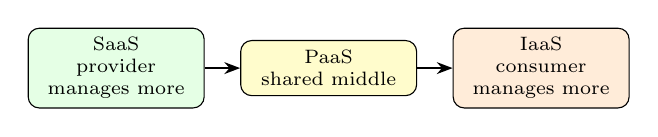
\begin{tikzpicture}[node distance=0.45cm]
\node[netbox, fill=green!10] (saas) {SaaS\\provider manages more};
\node[netbox, right=of saas, fill=yellow!20] (paas) {PaaS\\shared middle};
\node[netbox, right=of paas, fill=orange!15] (iaas) {IaaS\\consumer manages more};
\draw[netarrow] (saas) -- (paas);
\draw[netarrow] (paas) -- (iaas);
\end{tikzpicture}
\end{center}

\begin{block}{Security point}
The hospital never outsources accountability completely. It must understand which controls are run
by the provider and which remain the hospital's responsibility.
\end{block}
\end{frame}

\begin{frame}[c]{Deployment Models}
\begin{block}{Public cloud}
Cloud infrastructure is offered to many customers by a provider.
\end{block}

\begin{block}{Private cloud}
Cloud infrastructure is used exclusively by one organization.
\end{block}

\begin{block}{Community and hybrid cloud}
Community cloud is shared by organizations with common requirements. Hybrid cloud combines multiple
cloud or on-premises environments with portability or integration.
\end{block}
\end{frame}

\begin{frame}[c]{Cloud Actors}
\begin{block}{NIST reference architecture}
NIST describes five main actors: cloud consumer, cloud provider, cloud auditor, cloud broker, and
cloud carrier \cite{nist500292}.
\end{block}

\begin{exampleblock}{Hospital example}
St. Isidore is the consumer. The cloud platform is the provider. A security assessor may act as
auditor. A managed-service partner may broker or aggregate services. Network carriers provide
connectivity.
\end{exampleblock}
\end{frame}

\begin{frame}[c]{Cloud Security Threats}
\begin{block}{Typical risks}
Cloud introduces or amplifies risks such as abuse of cloud resources, insecure APIs, malicious
insiders, shared technology weaknesses, data loss, account hijacking, and unclear risk visibility.
\end{block}

\begin{exampleblock}{Hospital example}
A stolen cloud administrator account can expose backups, analytics datasets, network rules, or
identity settings. MFA and logging are not optional decorations; they are core controls.
\end{exampleblock}
\end{frame}

\begin{frame}[c]{Cloud Data Protection}
\begin{block}{Data states}
Health data must be protected in transit, at rest, and during use. Encryption helps, but key
management determines who can actually read the data.
\end{block}

\begin{block}{Trade-off}
Encrypting data before sending it to the cloud can reduce provider-insider risk, but may limit
server-side computation unless special techniques are used.
\end{block}
\end{frame}

\begin{frame}[c]{Security as a Service}
\begin{block}{Idea}
Cloud providers and security providers can offer identity management, data loss prevention, web and
email security, security assessments, intrusion management, SIEM, encryption, and continuity
services.
\end{block}

\begin{exampleblock}{Hospital example}
St. Isidore might use cloud email security to filter phishing, a SIEM to aggregate firewall and
identity logs, and cloud backup for disaster recovery.
\end{exampleblock}
\end{frame}

\takeawaysframe{
\begin{itemize}
    \item Cloud is still networking, identity, access control, encryption, logging, and contracts.
    \item Service model determines who controls which security layer.
    \item Healthcare cloud adoption requires explicit responsibility, auditability, and key-management decisions.
\end{itemize}
}{
St. Isidore can use cloud safely only if it understands provider responsibility, hospital
responsibility, data location, identity controls, and monitoring.
}

\section{Final Integration}
\sectiontitleframe{Final Integration}

\begin{frame}[c]{Final Concept Map}
\begin{center}
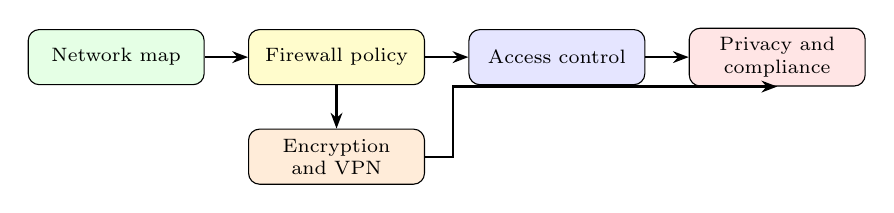
\begin{tikzpicture}[node distance=0.55cm]
\node[netbox, fill=green!10] (network) {Network map};
\node[netbox, right=of network, fill=yellow!20] (firewall) {Firewall policy};
\node[netbox, right=of firewall, fill=blue!10] (access) {Access control};
\node[netbox, below=of firewall, fill=orange!15] (crypto) {Encryption and VPN};
\node[netbox, right=of access, fill=red!10] (privacy) {Privacy and compliance};
\draw[netarrow] (network) -- (firewall);
\draw[netarrow] (firewall) -- (access);
\draw[netarrow] (firewall) -- (crypto);
\draw[netarrow] (access) -- (privacy);
\draw[netarrow] (crypto.east) -- ++(0.35,0) |- (privacy.south);
\end{tikzpicture}
\end{center}

\begin{block}{Reading the map}
The network map identifies possible paths. Firewall policy controls those paths. Access control
limits actions after reaching a system. Encryption protects traffic. Privacy and compliance
requirements shape how personal and health data must be protected in practice.
\end{block}
\end{frame}

\begin{frame}[c]{Final Recap}
\begin{block}{Core lesson}
Network security is not only blocking the Internet. It is designing and monitoring the expected
communication paths between hospital systems.
\end{block}

\begin{block}{Healthcare security lesson}
A well-designed hospital network makes clinical work possible while limiting unnecessary reachability,
containing compromise, preserving logs, and protecting patient data.
\end{block}
\end{frame}

\begin{frame}[allowframebreaks]{References}
\scriptsize
\bibliographystyle{apalike-AMS}
\bibliography{main}
\end{frame}

\end{document}
